\section{Compared regression techniques}
\label{sec:techs}

In the prediction of the development rate of the black Sigatoka, we
compare techniques such as least squares or ridge regression, commonly
encountered in the agricultural literature with machine learning
methods such as support vector regression, elastic regression and echo
state networks, where the parameter space of each technique is also
taken into account.

\subsection{Ordinary least squares regression}

Given a data set 
\begin{equation}
  D=\left\{(\vct{x}_i,y_i) \mid i=1\ldots n\right\}
\end{equation}
composed of the $d$-dimensional%
\footnote{Without loss of generality assume that the first component
  of every vector $\vct{x}_i$ is always $1$.}
%
feature vectors $\vct{x}_i\in\setR^d$ and the corresponding responses
$y_i$.
%
The ordinary least squares regression (OLSR) fits a linear model
$\tilde{y}_i = f(\vct{x}_i) = \vct{w}^T\vct{x}_i$ such that the sum of
squares of the residuals $(\tilde{y}_i-y_i)$ is minimized.
%
Let $\mat{X}$ be the $n\times{}d$ feature matrix containing the data
samples in its rows and $\vct{y}$ contain all the responses $y_i$
corresponding to each row, then the least squares regression finds
\begin{equation*}
  \hat{\vct{w}} =
  \arg\min_{\vct{w}}\left\| \mat{X}\vct{w} - \vct{y}\right\|_2^2
\end{equation*}
which is solved by means of the pseudoinverse
($\hat{\vct{w}}=\mat{X}^\dagger\vct{y}$) or equivalently by the singular
value decomposition of $\mat{X}$ \citep{Press2007}.

\TODO{Alex, no sé hasta donde hiciste en las pruebas ese ``arreglo''
  de que los datos tengan todos una entrada igual a 1.  De no ser así,
  el método no puede encontrar el offset, y sería como forzar que el
  modelo tenga que pasar por cero...}

\subsection{Ridge regression}

In contrast to the OLSR, the ridge regression (RR) adds a term to
penalize large weights \citep{scikitlearn2011}:
\begin{equation*}
\hat{\vct{w}} = 
\arg\min_{\vct{w}} \left\| \mat{X}\vct{w} - \vct{y} \right\|_2^2 + 
                 \alpha \left\|\vct{w}\right\|_2^2 
\end{equation*}
where the parameter $\alpha>0$ controls how strong is the shrinking of
the estimates towards zero.  This shrinkage introduces some bias but
helps to reduce the variance of the estimate.
%
The solution is given by $\hat{\vct{w}}=(\mat{X}^T\mat{X} +
\lambda\mat{I})^{-1}\mat{X}^T \vct{y}$.

\subsection{Support Vector Regression (SVR)}

\TODO{Estoy seguro que los lectores van a solicitar reducir esto y
  dejar solo la referencia.  No hay nada nuevo en el resto del paper
  que requiera toda esta información, así que hay que resumirlo a nada
  más lo esencial. }

From the perspective of Support Vector Regression (SVR) the regression
function is usually stated as 
\begin{equation}
\label{eq:svrfunc}
  \tilde{y} = f(\vct{x}) = \vct{w}^T\vct{x} + b
\end{equation}
The weights are selected in a convex optimization problem
\citep{Smola2004}:
\begin{align*}
  \text{minimize}   & \frac{1}{2}\|\vct{w}\|^2 + C\sum_{i=1}^n(\xi_i+\xi_i^\ast \\
  \text{subject to} & 
  \begin{cases}
    y_i - \vct{w}^T\vct{x}_i - b &\leq \epsilon + \xi_i    \\
    \vct{w}^T\vct{x}_i + b -y_i  &\leq \epsilon + \xi_i^\ast\\
    \xi_i,\xi_i^\ast               &\geq 0
  \end{cases}
\end{align*}
where $\epsilon$ is the maximal allowed deviation of the targets
$\tilde{y}_i$ from $y_i$, the slack variables $\xi_i$ and $\xi_i^\ast$
allow to cope with otherwise unfeasible constraints for the
optimization problem, and the constant $C>0$ controls the trade-off
between the flatness of $f$ and the tolerance to deviations larger
than $\epsilon$.

Note that since OLSR and RR use a squared error function, data
outliers will have a strong influence on the resulting weights
$\vct{w}$.  On the SVR formulation, however, the usage of the $L_1$
norm and the slack variables considerably restrict or completely block
the influence of those outliers.

The SVR problem is reformulated by means of the dual optimization
problem into
\begin{equation}
  \label{eq:svrw}
  \vct{w}=\sum_{i=1}^n(\alpha_i-\alpha_i^\ast)\vct{x}_i
\end{equation}
where $\alpha_i,\alpha_i^\ast\in[0,C]$ are Lagrange multipliers
subject to $\sum_{i=1}^n(\alpha_i-\alpha_i^\ast)=0$.
%
In this so-called \emph{Support Vector expansion} the weights are
expressed as a linear combination of the data set patterns
$\vct{x}_i$.
%
Inserting (\ref{eq:svrw}) in (\ref{eq:svrfunc}) leads to
\begin{equation}
  \label{eq:svrf}
 f(\vct{x}) = \sum_{i=1}^n(\alpha_i-\alpha_i^\ast)\vct{x}_i^T\vct{x} + b
\end{equation}
The Lagrange multipliers $\alpha_i,\alpha_i^\ast$ are both non-zero
only for those data points where $|f(\vct{x}_i) - y_i|\geq\epsilon$.
Hence, the expansion of $\vct{w}$ in terms of $\vct{x}_i$ is sparse.
Those data points with non-vanishing coefficients are called
\emph{Support Vectors} \citep{Wei2013}.

Additionally, in (\ref{eq:svrf}) it is possible to employ the
\emph{kernel trick} and replace the terms $\vct{x}_i^T\vct{x}$ with
the evaluation of any Mercer kernel
$k(\vct{x}_i,\vct{x})=\phi(\vct{x}_i)^T\phi(\vct{x})$, where
$\phi(\vct{x})$ is a non-linear mapping of the input space onto a
higher (even infinite) dimensional feature space.
%
The kernel evaluation draws unnecessary the explicit evaluation of the
non-linear mapping.
%
This allows to solve non-linear regressions in the input space by
implicitly mapping through the kernel the samples into the higher
dimensional space, where the linear regression occurs \citep{Alonso2013}.

\TODO{Habría que insertar aquí los kernels utilizados en los experimentos}

\subsection{Elastic-Net regression}

Elastic-Net is a linear regression model trained with $L1$ and $L2$ prior as regularizer. This combination allows for learning a sparse model where few of the weights are non-zero like Lasso, while still maintaining the regularization properties of Ridge  \citep{scikitlearn2011}. The convex combination of $L1$ and $L2$ is controled by using the $l1_{ratio}$ parameter.

Elastic-Net is useful when there are multiple features which are correlated with one another. Lasso is likely to pick one of these at random, while elastic-net is likely to pick both.
A practical advantage of trading-off between Lasso and Ridge is it allows Elastic-Net to inherit some of Ridge’s stability under rotation. The objective function to minimize is \citep{scikitlearn2011}:

$$\min_{w} { \frac{1}{2n_{samples}} \Bigr| \Bigr| Xw - y \Bigr| \Bigr|_2^2  + \alpha \rho \Bigr| \Bigr| w \Bigr| \Bigr|_1 + \frac{\alpha (1- \rho)}{2} \Bigr| \Bigr| w \Bigr| \Bigr|_2^2 } $$

\subsection{Echo State Networks (ESN)}
Recurrent Neural Networks (RNN) are useful for temporal patterns, but when they are trained with backpropagation methods, they are very slow.  Echo State Network (ESN) is an alternative training method to solve that problem.  ESN is based on the observation that if a random RNN possesses certain algebraic properties, training only a linear readout from it is often sufficient to achieve excellent performance in practical applications \citep{Lukose2009}. 
For a given training input signal $u(n)  \in R^{N_u}$ a desired target output signal $y^{target}(n) \in R^{N_y}$
is known. Here $n = 1, . . . ,T$ is the discrete time and $T$ is the number of data points in the training dataset. The task is to learn a model with output $y(n) \in R^{N_y}$, where $y(n)$ matches $y^target(n)$ as well as possible, minimizing an error measure $E(y,y^target)$, and, more importantly, generalizes well to unseen data. The untrained RNN part of an ESN is called a dynamical reservoir, and the resulting states x(n) are termed echoes of its input history \citep{Lukose2012}. Finally, these signals are sent to an output layer as shown in the \figref{figura3}.
\begin{figure}[h] 
 \centering
 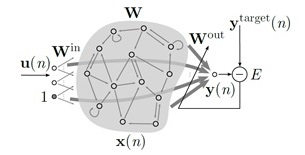
\includegraphics[scale=.9]{Reservorio}
 \caption{An echo state network \citep{Lukose2012}.} 
 \label{figura3} 
\end{figure}
 
The connections between the different elements of an Echo State Network have weights randomly generated. The weights of the internal connections of the reservoir $(W)$ as well as the weights of the input layer $(W_in)$, after being generated are set statically during all stages of implementation of the algorithm. The weights between the reservoir and the output layer $(W_out)$ are subject to changes of a supervised learning algorithm to correct the degree of error generated by the entire system \citep{Lukose2012}.
